% This is LLNCS.DOC the documentation file of
% the LaTeX2e class from Springer-Verlag
% for Lecture Notes in Computer Science, version 2.4
\documentclass{llncs}
\usepackage{llncsdoc}
\usepackage[T1]{fontenc}
\usepackage[utf8]{inputenc}
\usepackage{graphicx}
\graphicspath{ {Images/} }
%
\begin{document}
    \title{Context Aware Virtual Assistant with
    Case-Based Conflict Resolution in
    Multi-User Smart Home Environment}
    \author{Bauyrzhan Ospan\inst{1} \and Nawaz Khan \inst{2} \and Juan Augusto \inst{2} \and Mario Jose Quinde Li Say Tan \inst{2} \and Kenzhegali Nurgaliyev \inst{1}}
    \institute{Department of Information Technology, Kazakh University of Technology and Business, Kayim Muhamedhanov 37A, Astana 010000, Kazakhstan \\ \email{{bospan,knurgaliev}@nu.edu.kz}
    \and Department of Computer Science, Middlesex University, The Burroughs, London NW4 4BT, United Kingdom \\ \email{{N.X.Khan,J.Augusto,MQ093}@live.mdx.ac.uk}}
    \maketitle
    \begin{abstract}
        In this work we will examine and develop a Virtual Assistant which is the intelligence system that is used as a control
        interface of the Smart Home environment in the Farm Side Middlesex University laboratory. Specifically, the system is
        constructed to give multiple users ability to control devices` statuses by voice or text commands through the dialogue
        interface. Primarily, the main purpose of the system is to create user friendly interface with conflict resolution based
        on user cases. As a result, a Case-Based Reasoning algorithm was created with a k-Nearest Neighbor classification algorithm.
        In addition, Feed-Forward Artificial Neural Networks were used to classify user inputs, voice
        recognition and voice generation instruments were used to implement natural dialogue model of interactions with users.
        Moreover, the user friendly graphical web interface was developed. Further, a set of randomised double-blinded
        evaluation tests were established to check procedure of smart home control actions by multiple users.
    \end{abstract}
    \begin{keywords}
        Case-Based Reasoning, Context Awareness, Multiple User systems, Smart Home, Virtual Assistant
    \end{keywords}
    %
    \section{Introduction}
    %
    Managing a comfortable life could be a challenging task for people with special needs because some of them may need additional
    assistance to control electronic and electric devices in the living are [1]. The next group of users that probably seek
    assistance in Activities of Daily Life (ADL) is younger population while adults are away from home [1]. As a result,
    the Smart Home environments are developed to help users in controlling home and devices states with voice graphical
    interfaces [10] that are often called Virtual Assistants [1] or monitor behaviours of people
    with special needs [17] to classify changes in ADL that then alarm or notify relatives, health and care professionals
    and organizations [9]. Additional finding identified other techniques in the state of art.
    For example, in Smart Home systems there are Ontology-based platforms that allows to analyze user`s actions and
    perform context recognition [14] or visual tools for creating personal preferences table of each user based on semantics
    metadata [11]. As a consequence, majority of the researches is aimed to develop systems that helps alone living users.\\
    Despite number of
    researches in the Smart Home solutions that are automated, adaptive, multifunctional and interactive, there is a lack of
    investigations and development of systems that operates in a conflict resolution between multiple users with different
    needs and priorities. Some researchers in order to solve this dilemma developed context-aware automation platforms
    [13, 16] that resolves conflicts between automated devices such as fire alarms and automated door locks.
    On the other hand, these solutions resolves conflicts only between automated devices based on priorities of their rules.
    The next group of
    developers are focused on preference Rule-Based Reasoning (RBR) to resolve conflicts between users [1]. Even through
    these systems introduces efficient set of rules, they are not able to handle with adaptation to the new user cases or
    specific out-of-rule situations. \\
    To sum up
    state of art, there are number of systems that monitors and adapts to single users, resolves conflicts between devices
    in single user multi-agent environments and resolves conflicts between users based on if-else rules. On the contrary,
    there is a lack of the Virtual Assistants with an adaptive conflict resolution systems.\\
    In this research, we propose a Virtual Assistant (VA) system that controls Smart Home environment based on the user inputs via
    voice and text based dialogue graphical web user interface for multiple users. As a result, we developed number of
    subsystems to fully implement number of requests. First of all, interaction with the VA has to be user-friendly and
    natural as a human to human interaction. Second, the system has to be able to control and monitor state of the Smart
    Home devices. Finally, the VA has to manage to resolve conflicts between multiple users, and adapt to the new user cases.\\
    To cover all objectives, we introduced and developed the VA with next modules. Firstly, we have developed user friendly
    graphical interface based on web and cloud technologies to give to user intuitive way of interacting with the VA. For this
    reason, we used dynamic web framework, cloud voice recognition and generation technologies and animated emotional icons
    to mimicry natural face emotions in the dialogues. In addition to user friendly interface, we have developed and implemented
    adaptive natural language classification algorithms based on Artificial Neural Network (ANN) to make the VA understand
    different variates of the user commands and argumentation sentences, because they are effective algorithms for
    sentence classification [19]. Therefore, users were able to speak to
    VA in the way they speak with other human. Secondly, we used Farm Side Middlesex University Smart Home laboratory and
    Smart Home devices control unit to manage and monitor Smart Home devices. In order that, we have developed and integrated
    software API to implement communication between Smart Home control unit and VA. The last but not the least, we have
    introduced and developed a conflict resolution system that used Case-Based Reasoning (CBR) to make a decision about
    conflict between multiple users. In order to make decision, VA identifies in dialogue form the argumentation of the user
    in performing an action, analyzes via k-nearest neighbour (kNN) algorithm similarities between
    this case and previous cases and chooses best-fit case [4,7,15]. In other words, VA asks user to say why he or she wants to change
    device status if there conflicting instruction from other user and makes decision what to do with device based on users
    arguments and previous cases. Futhermore, arguments priorities was established by personal user preferences [3] because
    number of researches shows that the preference-based argumentation increases ability of the systems to meet user
    expectations [5].\\
    Furthermore, we have established randomized double-blinded evaluation tests. In order to perform randomized double
    blinded experiment, we developed scenario creating sub-module. Firstly, it creates random scenario for tester by choosing
    conflicting device and arguments for tester by using crypto-secure randomise function based on operation system inner
    clocks. Secondly, it provides such instructions to testers that he or she was
    asked to provide command and arguments in their own words. As a result, it was hidden from us and testers scenarios till
    the beginning of the experiment. In addition, testers were asked to fill evaluation form. To conclude, feedback from
    testers are positive and only weak place of the system is accent recognition task.\\
    This paper presents Virtual Assistant in the multiple user Smart Home environment. The Virtual Assistant was created
    to manage and monitor Smart Home environment by dialogue based interaction with users. Different machine learning
    algorithms and cloud technologies were implemented to meet project objectives. The main focus of the research was to
    develop adaptive conflict resolution system based on Case-Based Reasoner. The validation tests feedback is positive.
    The future direction of the work is to implement context-aware system that analyzes user behaviour and reports it as
    a case to the database of Case-Based Reasoner.\\
    This paper presents Virtual Assistant in the multiple user Smart Home environment. The architecture of the system is
    described in the Section II. The system algorithms and sequences are described in the Section III. Section IV demonstrates
    our results and validation. Finally, Section V draws the conclusion and predictions for the future work.
    %
    \section{Architecture}
    %
    Technical details of the system are given in this section.
    It consider architecture diagram of the system and explanation of all functional units called modules each
    or divided into the groups called components.
    \subsection{Overall}
    The architecture of the system is layered and modular.
    As a result, each functional part (module) of the system is designed to execute complete task and some of them are
    divided into components.
    The component is group of modules that performs complex task that consists of a number of simple tasks.
    For example, Order Classification and Reason Classification modules are grouped to Classification component.\\
    In addition, in order to give better understanding of the system, the architecture is divided into layers.
    Layer is functional components of the system that sequentially divides it into hierarchical groups that
    communicates only with layer above or layer below except Database layer.
    For example, Cloud API layer is consists of Speech Generation and Speech Recognition that communicate only with
    Front End layer and Core layer.\\
    Layer is demonstrated as white rectangle with grey icon and name in it.
    Web pages of the web interface is demonstrated as white colored box with blue drawing and text in it.
    Hexagonal icon with white image inside colored blue and text below is module of the system.
    White quadrilateral with grey illustration of device and it`s name underneath is icon of electronic device driven
    by Smart Home environment.
    Colored rectangle with text in the bottom right corner is illustration of components.
    All communication inside the system is demonstrated as arrows in the Fig.1.
    \footnote{Communication types and lifelines of the system is described in the Section III.}
    \begin{figure}
        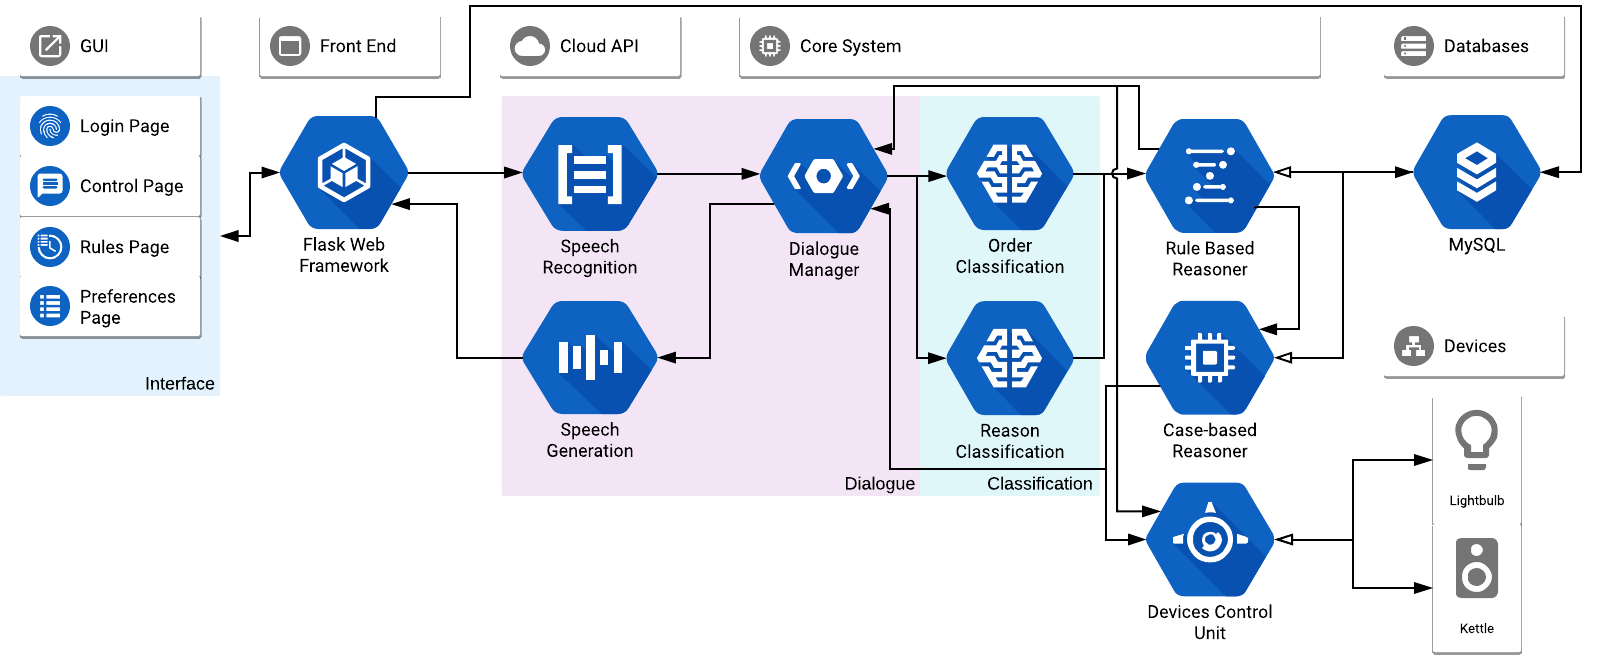
\includegraphics[width=\textwidth]{arch.png}
        \caption[]{Architecture diagram of the system}
    \end{figure}
    \subsection{Graphical User Interface and Front End}
    The interface of the system is graphical web interface developed as web site.
    As a result, Graphical User Interface (GUI) is expressed by 3 functional and Login Pages that are listed below:
    \begin{enumerate}
        \item Login Page: Welcome interface - user chooses his or her account.
        \item Control Page: Dialogue interface - user communicates with system in form of dialogue by voice or text chat,
        gives orders \footnote{Order is command of the user given to the system. For example, turn off the light.} and reasons \footnote{Reason is argument given by the user to the system to justify his/her order. For example, turn off the light, because my eyes hurts.}.
        \item Rules \footnote{Rule is set of instructions given for system to do automatically. For example, system is obligated keep kettle turned off from 11:00 till 13:00 everyday because of energy saving issue.}
        Page: Rules editing interface - user edits list of instructions \footnote{Rules are discussed in the Section III.} given to the system.
        \item Preferences \footnote{Preference is set of issues that justifies orders of the user to the system. Every user type has its own priority level for preferences.} Page: Preferences editing interface - user edits his or her preferences \footnote{Preferences are discussed in the Section III.}.
    \end{enumerate}
    Flask Micro Web Framework is used as Front End controlling technology or Back End of the interface, because most of the project is coded by Python 3 language.
    \subsection{Cloud API}
    The function units of the Speech Generation and Speech Recognition were established via W3C Web Speech API \footnote{More information on https://w3c.github.io/speech-api/speechapi.html.}.
    They are JavaScript Application Programming Interfaces (API) that are used by most of the modern browsers.
    As a result, the system sends record of the user input to W3C API and it returns text that is the recognition of the record.
    Moreover, the system sends text to the browser of the user in such way that the browser automatically generates it into voice.
    The modules of the Speech Generation and Speech Recognition are inserted to the Dialogue component with Dilague Manager module.
    \subsection{Core System}
    Core System is main functional layer of the system.
    Consequently, functions as decision-making, dialogue compilation, text classification and device controlling are all executed in the modules inside the Core System layer.
    It consists of Dialogue Manager, Classification Component, Rule-Based Reasoner, Case-Based Reasoner and Device Control Unit.
    \subsection{Dialogue Manager}
    Dialogue Manager is one of the central modules of the system.
    Dialogue Manager receives phrases from the user and classifies it by Classification component and sends it to Rule-Based Reasoner.
    Based on the data from Rule-Based Reasoner and actions done by the system it sends human readable report or response to user via interface.
    In addition to Cloud API, Dialogue Manager is part of the Dialogue component that is the subsystem to communicate with user in natural way.
    Lastly, Dialogue Manager is set of if-else rules and dialogues database developed to pretend human-like speaking.
    \subsection{Classification Component}
    Classification component is group of two Classification modules that are Order and Reason Classification.
    Their function is to classify orders and reason from user input raw data.
    As a result, they need classification algorithm.\\
    Text classification is non-trivial complex task that is cannot be solved sequentially or by sequential algorithms artificial neural network systems (ANN) provides the better solution \cite{14}.
    Backpropagation as an ANS is very useful in recognizing complex patterns and performing nontrivial mapping functions.
    The figure below represents a simple Feed Forward Neural Network (FNN) diagram.
    The rounded objects represent the artificial neurons or processing elements of a neural network.
    The directed lines that are connecting the neurons are called weights that are the multiplication coefficients for input signal.
    Also every line of processing elements is a layer of a network.
    \begin{figure}
        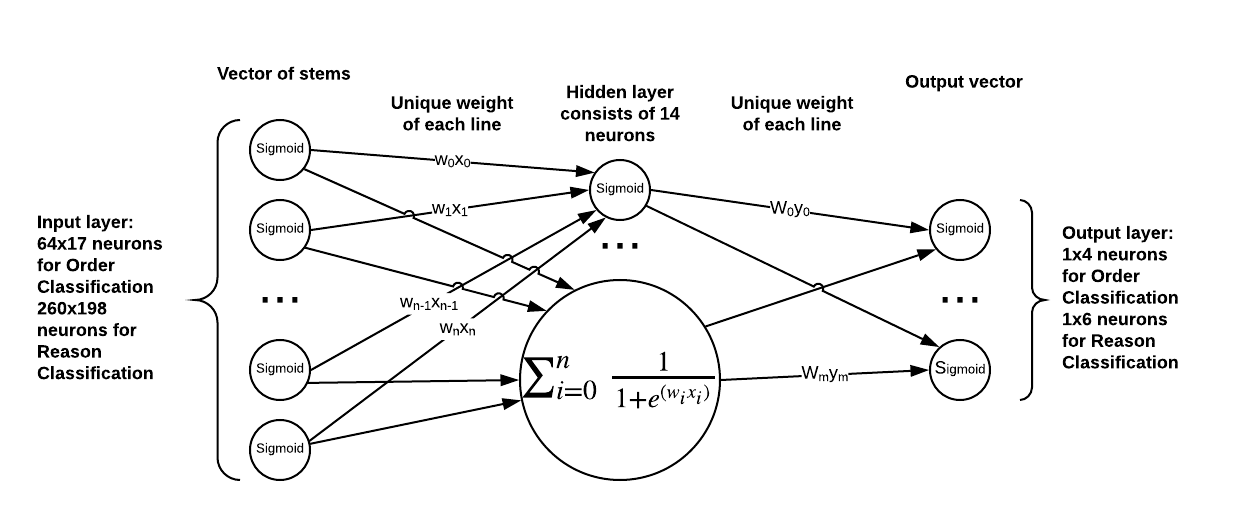
\includegraphics[width=\textwidth]{ANN.png}
        \caption[]{Classification Neural Network Topology}
    \end{figure}
    \subsubsection{Topology of the Artificial Neural Network} is consists of Input, Output and Hidden layers.\\
    \em Input layer \em consist of input neurons that are binomial representation of the unique stemmed words (stemmed by LancasterStemmer from Natural Language Toolkit library) inside the text that is already cleaned from punctuation and meaningless words like articles.
    In a text document a word may exist in a different morphological variants.
    For example the word “love” may also exist in other morphological variants such as “loving”, “loved”.
    While these morphological variants are different word forms, that represent same concept.
    In text categorization and other similar tasks it is desirable to combine these morphological variants of the same word into one canonical form and represent it like vector that is called stemmed version.\\
    \em Output layer \em gives vector of possibilities that the text is inside of classes \footnote{Class is the group of reasons for Reason Classification and group of orders for Order Classification.}.
    The most possible class is the classification answer of the neural network.\\
    \em Hidden layer \em is the regression function of FNN, or layer between input and output layers.
    FNN applies a sequence of linear functions to the data.
    These functions are sigmoid linear transformation of the previous layer.
    As a result, it followed by a squashing nonlinearity
    While training the ANN (see below) it was concluded that the accuracy of the neural network does not significantly changes between one hidden layer neural network and multiple hidden layer neural network.
    The most efficient number of hidden layer neurons (14) was found by calculation of the delta that was calculated by 1000 iterations of Backpropogation training algorithm with standard training/test set especially created for this experiment.
    \begin{figure}
        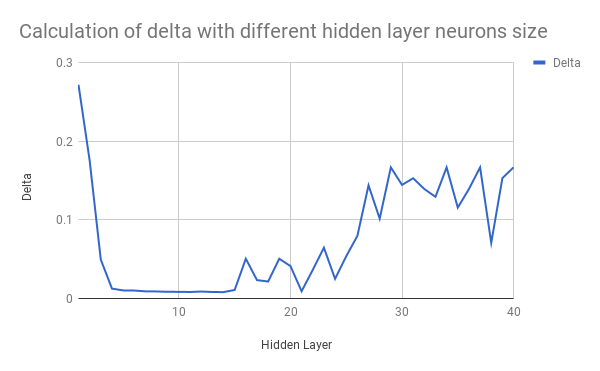
\includegraphics[width=0.8\textwidth]{HL.png}
        \caption[]{Iterations of FNN with different Hidden Layer size, where horizontal line is number of neurons and vertical line is delta function percentage}
    \end{figure}
    \subsubsection{General Case: Trivial Reason.}
    In the next example user typed that he wants to change device status because he needs to finish a project about flu.
    Classifier says that it is 99.9\% about work, and a little bit (0.05\%) about heath issue, because his project about flu.
    The system normally does not accept any classification lower that 80\% possibility, and if user says something not
    correlated to the predefined preferences, the system will skip classification and ask again.
    \begin{example}
        User input is: \em I need to finish my project about flu \em \\
        System classified it as: \em [['Work', 0.99951473383654765], ['Health', 0.056650409249493161], ['Entertainment', 0.0011293354032656073], ['Energy', 1.4169164768812246e-05], ['Security', 1.238332260956378e-05], ['Food', 3.1674436013529605e-07]] \em
    \end{example}
    \subsubsection{General Case: Nontrivial Reason.}
    In the next example user typed "G'ylym janyp turg'an s'yraq" (Kazakh Language: Science is a burning candle).
    The system did not managed to classify this reason, because the system is tuned only for English.
    \begin{example}
        User input is: \em G'ylym janyp turg`an s`yraq \em\\
        System classified it as: \em [] (Null) \em
    \end{example}
    \subsection{Training of FNN}
    It was used Backpropogation method for artificial neural network weights of the synapses optimisation.
    The Backpropagation learning rule based on supervised learning \cite{14}.
    In order to train neural network, a set of training documents and a specification of the pre-defined categories the documents belong to are required.
    Training and testing sets were created specially for this experiment.
    There were used common English phrases and their synonyms to create set of sentences and their class.
    During training, the connection weights of the neural network are initialized to random values.
    The training examples in the training set are then presented to the neural network classifier in random order, and the connection weights are adjusted according to the Backpropagation learning rule.
    This process is repeated until the learning error falls below a predefined tolerance level (99.95\%).
    Below there is an example of the training of the Reason Classifier.
    \begin{example}
        Input matrix: 260x198 Output matrix: 1x6\\
        delta after 10000 iterations:0.00195103818538\\
        delta after 20000 iterations:0.00132469839464\\
        delta after 30000 iterations:0.00105975676227\\
        delta after 40000 iterations:0.000905619354028\\
        delta after 50000 iterations:0.000802125845806\\
        delta after 60000 iterations:0.000726645045015\\
        delta after 70000 iterations:0.000668536139359\\
        delta after 80000 iterations:0.000622059862315\\
        delta after 90000 iterations:0.000583815748815\\
        delta after 100000 iterations:0.000551645861196\\
        saved synapses to: ./include/synapses.json\\
        processing time: 103.20042490959167 seconds\\
    \end{example}
    \subsection{Rule-Based Reasoner}
    Rule-Based Reasoner receives data about the user`s order and compares it with rules in the Database and actual status of the devices.
    Core of the Rule-Based Reasoner is the set of if-else rules:
    \begin{enumerate}
        \item If status of device equals to status that user already wants: return similarity response; else: go further.
        \item If there is conflict between rule and user`s order: send task to Case-Based Reasoner; else: send command to Device COntrol Unit.
    \end{enumerate}
    \subsection{Case-Based Reasoner}
    Case-Based Reasoner works by finding the lowest distance of input case to the cases inside the database.
    CBR is an artificial intelligence approach to determine a similarity amongst a set of cases.
    This method indexes cases from history of the system usage and retrieves best similar case by measurement of distance between the input case and past cases.
    The result of finding best match is stored inside the cases database to update the cases database and adapt old solution to the new variables and environment.
    CBR is based on a suggestion that the similar cases have similar solution.
    The decisions in our system is binary (0 for not change device status, 1 for change it).
    As a result, it is accessible that CBR assumption works in our system.
    Most of the CBR systems uses k-nearest neighbour algorithm.
    The accuracy of this classification algorithm seriously depends on the metrics or system of measurement used to compute distances between different cases.
    The nearest neighbour algorithm determines the similarity or dissimilarity of a new case with the case base and follows a cyclical process of Retrieve-Reuse-Revise-Retain.
    In our case inputs to the system are in different system of measurements.
    Cases in the system are build on preferences and priority of users of the system.
    Both two variables have different basis.
    As a result, standard Euclidean Distance cannot be used as a distance measurement algorithm.
    It was proposed to use Mahalanobis distance that is the global linear transformation tool of the input spaces of the cases from different classes separated by a large margins.
    Using of Mahalanobis distance significantly increases kNN accuracy.
    In addition, there was used a Genetic Algorithm to find best value of Mahalanobis covariance matrix.
    It is was set nearly 11 quadrillion types of mutations patterns.
    The covariance matrix was used as genome of each genome in the epoch.
    As a result, each epoch system chooses best accuracy model and mutates it`s one hundred children with different not significant mutations in the genome.
    Then the system iterate again while accuracy of the best model (king) will not reach threshold value.
    \subsection{Device Control Unit}
    Smart Home environment of the Farm Side Middlesex University is driven by Vera Secure system.
    In consequence, we developed API to communicate with it.
    Vera Secure system has own web interface.
    In order to communicate with it, we sending and receiving GET and POST requests.
    Special POST requests changes status of the devices, which are kettle and light in our experiment.
    Next, updating information about device statuses is done by parsing response from special GET request sent to the Vera Secure server.
    \section{Sequences}
    %
    Sequences inside the system are mentioned in this chapter.
    \subsection{Terminology}
    We used user types and preference system proposed by \cite{9} .
    As a result, different group of users were outlined and divided by age.
    Moreover, we declared updated system of preferences.
    \begin{table}
        \caption{List of users and preferences}
        \begin{tabular}{llllll}
            \hline\noalign{\smallskip}
            User types & Preferences (positions 0,1,2,3,4,5)\\
            \noalign{\smallskip}
            \hline
            \noalign{\smallskip}
            Adult (26-69 ages) & Security, Health, Work, Food, Energy, Entertainment\\
            Elderly (older 70) & Health, Security, Food, Energy, Entertainment, Work\\
            Young (up to 25 ages) & Security, Work, Entertainment, Health, Food, Energy\\
            \hline
        \end{tabular}
    \end{table}

    \subsection{Regular Case}
    \subsection{Conflicting Case}
    \section{Results and Validation}
    %
    \section{Conclution}
    \section{References}
    \begin{thebibliography}{1}
        \bibitem {1}
        Alirezaie, M., Renoux, J., Köckemann, U., Kristoffersson, A., Karlsson, L., Blomqvist, E., Tsiftes, N., Voigt, T., Loutfi, A.: An Ontology-based Context-aware System for Smart Homes: E-care@home. Sensors. 17, 1586 (2017).

        \bibitem {2}
        Aztiria, A., Augusto, J., Basagoiti, R., Izaguirre, A., Cook, D.: Learning Frequent Behaviors of the Users in Intelligent Environments. IEEE Transactions on Systems, Man, and Cybernetics: Systems. 43, 1265-1278 (2013).

        \bibitem {3}
        Fleury, A., Vacher, M., Noury, N.: SVM-Based Multimodal Classification of Activities of Daily Living in Health Smart Homes: Sensors, Algorithms, and First Experimental Results. IEEE Transactions on Information Technology in Biomedicine. 14, 274-283 (2010).

        \bibitem {4}
        Göynügür, E., Bernardini, S., de Mel, G., Talamadupula, K., Şensoy, M.: Policy Conflict Resolution in IoT via Planning. Advances in Artificial Intelligence. 169-175 (2017).

        \bibitem {5}
        Hadj, R., Hamon, C., Chollet, S., Vega, G., Lalanda, P.: Context-based conflict management in pervasive platforms. 2017 IEEE International Conference on Pervasive Computing and Communications Workshops (PerCom Workshops). (2017).

        \bibitem {6}
        Kabir, M., Hoque, M., Seo, H., Yang, S.: Machine Learning Based Adaptive Context-Aware System for Smart Home Environment, https://pdfs.semanticscholar.org/8cf5/fe5062727744f5429bb34d9c0bd24f439ee6.pdf.

        \bibitem {7}
        Khan, N., Alegre, U., Kramer, D., Augusto, J.: Is ‘Context-Aware Reasoning = Case-Based Reasoning’?. Modeling and Using Context. 418-431 (2017).

        \bibitem {8}
        Mayer, S., Inhelder, N., Verborgh, R., Van de Walle, R., Mattern, F.: Configuration of smart environments made simple: Combining visual modeling with semantic metadata and reasoning. 2014 International Conference on the Internet of Things (IOT). (2014).

        \bibitem {9}
        Nurgaliyev, K., Mauro, D., Khan, N., Augusto, J.: Improved Multi-user Interaction in a Smart Environment Through a Preference-Based Conflict Resolution Virtual Assistant. 2017 International Conference on Intelligent Environments (IE). (2017).

        \bibitem {10}
        Oguego, C., Augusto, J., Muñ`oz, A., Springett, M.: A survey on managing users’ preferences in ambient intelligence. Universal Access in the Information Society. (2017).

        \bibitem {11}
        Oguego, C., Augusto, J., Muñoz, A., Springett, M.: Using argumentation to manage users’ preferences. Future Generation Computer Systems. 81, 235-243 (2018).

        \bibitem {12}
        Ospan, B.: Simulation of a Simple Bio-Mimetic Robot with Neuromorphic Control System and Optimization Based on the Genetic Algorithm. International Journal of Innovations in Engineering and Technology. 8, 59-65 (2017).
        \bibitem {13}
        Portet, F., Vacher, M., Golanski, C., Roux, C., Meillon, B.: Design and evaluation of a smart home voice interface for the elderly: acceptability and objection aspects. Personal and Ubiquitous Computing. 17, 127-144 (2011).

        \bibitem {14}
        Ramasundaram, S., Victor, S.: Text Categorization by Backpropagation Network, http://www.ijcaonline.org/archives/volume8/number6/1217-1754.

        \bibitem {15}
        Reichherzer, T., Satterfield, S., Belitsos, J., Chudzynski, J., Watson, L.: An Agent-Based Architecture for Sensor Data Collection and Reasoning in Smart Home Environments for Independent Living. Advances in Artificial Intelligence. 15-20 (2016).

        \bibitem {16}
        Siolas, G., Caridakis, G., Mylonas, P., Kollias, S., Stafylopatis, A.: Context-Aware User Modeling and Semantic Interoperability in Smart Home Environments. 2013 8th International Workshop on Semantic and Social Media Adaptation and Personalization. (2013).

        \bibitem {17}
        Weinberger, K., Lawrence, S.: Distance Metric Learning for Large Margin Nearest Neighbor Classification. Journal of Machine Learning Research. 10, 207-244 (2009).

    \end{thebibliography}

\end{document}